\documentclass[twoside]{book}

% Packages required by doxygen
\usepackage{fixltx2e}
\usepackage{calc}
\usepackage{doxygen}
\usepackage[export]{adjustbox} % also loads graphicx
\usepackage{graphicx}
\usepackage[utf8]{inputenc}
\usepackage{makeidx}
\usepackage{multicol}
\usepackage{multirow}
\PassOptionsToPackage{warn}{textcomp}
\usepackage{textcomp}
\usepackage[nointegrals]{wasysym}
\usepackage[table]{xcolor}

% Font selection
\usepackage[T1]{fontenc}
\usepackage[scaled=.90]{helvet}
\usepackage{courier}
\usepackage{amssymb}
\usepackage{sectsty}
\renewcommand{\familydefault}{\sfdefault}
\allsectionsfont{%
  \fontseries{bc}\selectfont%
  \color{darkgray}%
}
\renewcommand{\DoxyLabelFont}{%
  \fontseries{bc}\selectfont%
  \color{darkgray}%
}
\newcommand{\+}{\discretionary{\mbox{\scriptsize$\hookleftarrow$}}{}{}}

% Page & text layout
\usepackage{geometry}
\geometry{%
  a4paper,%
  top=2.5cm,%
  bottom=2.5cm,%
  left=2.5cm,%
  right=2.5cm%
}
\tolerance=750
\hfuzz=15pt
\hbadness=750
\setlength{\emergencystretch}{15pt}
\setlength{\parindent}{0cm}
\setlength{\parskip}{3ex plus 2ex minus 2ex}
\makeatletter
\renewcommand{\paragraph}{%
  \@startsection{paragraph}{4}{0ex}{-1.0ex}{1.0ex}{%
    \normalfont\normalsize\bfseries\SS@parafont%
  }%
}
\renewcommand{\subparagraph}{%
  \@startsection{subparagraph}{5}{0ex}{-1.0ex}{1.0ex}{%
    \normalfont\normalsize\bfseries\SS@subparafont%
  }%
}
\makeatother

% Headers & footers
\usepackage{fancyhdr}
\pagestyle{fancyplain}
\fancyhead[LE]{\fancyplain{}{\bfseries\thepage}}
\fancyhead[CE]{\fancyplain{}{}}
\fancyhead[RE]{\fancyplain{}{\bfseries\leftmark}}
\fancyhead[LO]{\fancyplain{}{\bfseries\rightmark}}
\fancyhead[CO]{\fancyplain{}{}}
\fancyhead[RO]{\fancyplain{}{\bfseries\thepage}}
\fancyfoot[LE]{\fancyplain{}{}}
\fancyfoot[CE]{\fancyplain{}{}}
\fancyfoot[RE]{\fancyplain{}{\bfseries\scriptsize Generated by Doxygen }}
\fancyfoot[LO]{\fancyplain{}{\bfseries\scriptsize Generated by Doxygen }}
\fancyfoot[CO]{\fancyplain{}{}}
\fancyfoot[RO]{\fancyplain{}{}}
\renewcommand{\footrulewidth}{0.4pt}
\renewcommand{\chaptermark}[1]{%
  \markboth{#1}{}%
}
\renewcommand{\sectionmark}[1]{%
  \markright{\thesection\ #1}%
}

% Indices & bibliography
\usepackage{natbib}
\usepackage[titles]{tocloft}
\setcounter{tocdepth}{3}
\setcounter{secnumdepth}{5}
\makeindex

% Hyperlinks (required, but should be loaded last)
\usepackage{ifpdf}
\ifpdf
  \usepackage[pdftex,pagebackref=true]{hyperref}
\else
  \usepackage[ps2pdf,pagebackref=true]{hyperref}
\fi
\hypersetup{%
  colorlinks=true,%
  linkcolor=blue,%
  citecolor=blue,%
  unicode%
}

% Custom commands
\newcommand{\clearemptydoublepage}{%
  \newpage{\pagestyle{empty}\cleardoublepage}%
}

\usepackage{caption}
\captionsetup{labelsep=space,justification=centering,font={bf},singlelinecheck=off,skip=4pt,position=top}

%===== C O N T E N T S =====

\begin{document}

% Titlepage & ToC
\hypersetup{pageanchor=false,
             bookmarksnumbered=true,
             pdfencoding=unicode
            }
\pagenumbering{alph}
\begin{titlepage}
\vspace*{7cm}
\begin{center}%
{\Large Lab Assignment -\/3 \\[1ex]\large 1 }\\
\vspace*{1cm}
{\large Generated by Doxygen 1.8.13}\\
\end{center}
\end{titlepage}
\clearemptydoublepage
\pagenumbering{roman}
\tableofcontents
\clearemptydoublepage
\pagenumbering{arabic}
\hypersetup{pageanchor=true}

%--- Begin generated contents ---
\chapter{File Index}
\section{File List}
Here is a list of all files with brief descriptions\+:\begin{DoxyCompactList}
\item\contentsline{section}{L3/\hyperlink{bus_8tcl}{bus.\+tcl} }{\pageref{bus_8tcl}}{}
\item\contentsline{section}{L3/\hyperlink{_q1_8c}{Q1.\+c} }{\pageref{_q1_8c}}{}
\item\contentsline{section}{L3/\hyperlink{_q2__client_8c}{Q2\+\_\+client.\+c} }{\pageref{_q2__client_8c}}{}
\item\contentsline{section}{L3/\hyperlink{_q2__server_8c}{Q2\+\_\+server.\+c} }{\pageref{_q2__server_8c}}{}
\item\contentsline{section}{L3/\hyperlink{ring_8tcl}{ring.\+tcl} }{\pageref{ring_8tcl}}{}
\item\contentsline{section}{L3/\hyperlink{star_8tcl}{star.\+tcl} }{\pageref{star_8tcl}}{}
\end{DoxyCompactList}

\chapter{File Documentation}
\hypertarget{bus_8tcl}{}\section{L3/bus.tcl File Reference}
\label{bus_8tcl}\index{L3/bus.\+tcl@{L3/bus.\+tcl}}
\subsection*{Functions}
\begin{DoxyCompactItemize}
\item 
\hyperlink{bus_8tcl_a30728837c246b65ef76298af0101d99c}{finish}
\end{DoxyCompactItemize}


\subsection{Function Documentation}
\mbox{\Hypertarget{bus_8tcl_a30728837c246b65ef76298af0101d99c}\label{bus_8tcl_a30728837c246b65ef76298af0101d99c}} 
\index{bus.\+tcl@{bus.\+tcl}!finish@{finish}}
\index{finish@{finish}!bus.\+tcl@{bus.\+tcl}}
\subsubsection{\texorpdfstring{finish()}{finish()}}
{\footnotesize\ttfamily finish}



Definition at line 13 of file bus.\+tcl.


\hypertarget{_q1_8c}{}\section{L3/\+Q1.c File Reference}
\label{_q1_8c}\index{L3/\+Q1.\+c@{L3/\+Q1.\+c}}
{\ttfamily \#include $<$stdio.\+h$>$}\newline
{\ttfamily \#include $<$string.\+h$>$}\newline
Include dependency graph for Q1.\+c\+:
\nopagebreak
\begin{figure}[H]
\begin{center}
\leavevmode
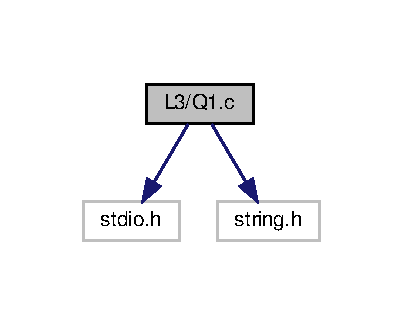
\includegraphics[width=194pt]{_q1_8c__incl}
\end{center}
\end{figure}
\subsection*{Functions}
\begin{DoxyCompactItemize}
\item 
char \hyperlink{_q1_8c_a874c2affa0e05eef5dbcd62f0232a591}{find\+Class} (char str\mbox{[}$\,$\mbox{]})
\item 
void \hyperlink{_q1_8c_a5f90e3b26836b8a0ff338c925198593d}{separate} (char str\mbox{[}$\,$\mbox{]}, char ip\+Class)
\item 
int \hyperlink{_q1_8c_ae66f6b31b5ad750f1fe042a706a4e3d4}{main} ()
\end{DoxyCompactItemize}


\subsection{Function Documentation}
\mbox{\Hypertarget{_q1_8c_a874c2affa0e05eef5dbcd62f0232a591}\label{_q1_8c_a874c2affa0e05eef5dbcd62f0232a591}} 
\index{Q1.\+c@{Q1.\+c}!find\+Class@{find\+Class}}
\index{find\+Class@{find\+Class}!Q1.\+c@{Q1.\+c}}
\subsubsection{\texorpdfstring{find\+Class()}{findClass()}}
{\footnotesize\ttfamily char find\+Class (\begin{DoxyParamCaption}\item[{char}]{str\mbox{[}$\,$\mbox{]} }\end{DoxyParamCaption})}

Function to find out the Class \begin{DoxyAuthor}{Author}
Aman Jaiswal 
\end{DoxyAuthor}

\begin{DoxyParams}{Parameters}
{\em str\+:-\/} & ip address as string \\
\hline
\end{DoxyParams}
\begin{DoxyDate}{Date}
22/08/2019 
\end{DoxyDate}


Definition at line 19 of file Q1.\+c.

\mbox{\Hypertarget{_q1_8c_ae66f6b31b5ad750f1fe042a706a4e3d4}\label{_q1_8c_ae66f6b31b5ad750f1fe042a706a4e3d4}} 
\index{Q1.\+c@{Q1.\+c}!main@{main}}
\index{main@{main}!Q1.\+c@{Q1.\+c}}
\subsubsection{\texorpdfstring{main()}{main()}}
{\footnotesize\ttfamily int main (\begin{DoxyParamCaption}{ }\end{DoxyParamCaption})}



Definition at line 149 of file Q1.\+c.

\mbox{\Hypertarget{_q1_8c_a5f90e3b26836b8a0ff338c925198593d}\label{_q1_8c_a5f90e3b26836b8a0ff338c925198593d}} 
\index{Q1.\+c@{Q1.\+c}!separate@{separate}}
\index{separate@{separate}!Q1.\+c@{Q1.\+c}}
\subsubsection{\texorpdfstring{separate()}{separate()}}
{\footnotesize\ttfamily void separate (\begin{DoxyParamCaption}\item[{char}]{str\mbox{[}$\,$\mbox{]},  }\item[{char}]{ip\+Class }\end{DoxyParamCaption})}

Function to separate Network ID as well as Host ID and print them \begin{DoxyAuthor}{Author}
Aman Jaiswal 
\end{DoxyAuthor}

\begin{DoxyParams}{Parameters}
{\em str\+:-\/} & ip address as string,and class of ip adress \\
\hline
\end{DoxyParams}
\begin{DoxyDate}{Date}
22/08/2019 
\end{DoxyDate}


Definition at line 68 of file Q1.\+c.


\hypertarget{_q2__client_8c}{}\section{L3/\+Q2\+\_\+client.c File Reference}
\label{_q2__client_8c}\index{L3/\+Q2\+\_\+client.\+c@{L3/\+Q2\+\_\+client.\+c}}
{\ttfamily \#include $<$arpa/inet.\+h$>$}\newline
{\ttfamily \#include $<$netinet/in.\+h$>$}\newline
{\ttfamily \#include $<$stdio.\+h$>$}\newline
{\ttfamily \#include $<$stdlib.\+h$>$}\newline
{\ttfamily \#include $<$string.\+h$>$}\newline
{\ttfamily \#include $<$sys/socket.\+h$>$}\newline
{\ttfamily \#include $<$sys/types.\+h$>$}\newline
{\ttfamily \#include $<$unistd.\+h$>$}\newline
Include dependency graph for Q2\+\_\+client.\+c\+:
\nopagebreak
\begin{figure}[H]
\begin{center}
\leavevmode
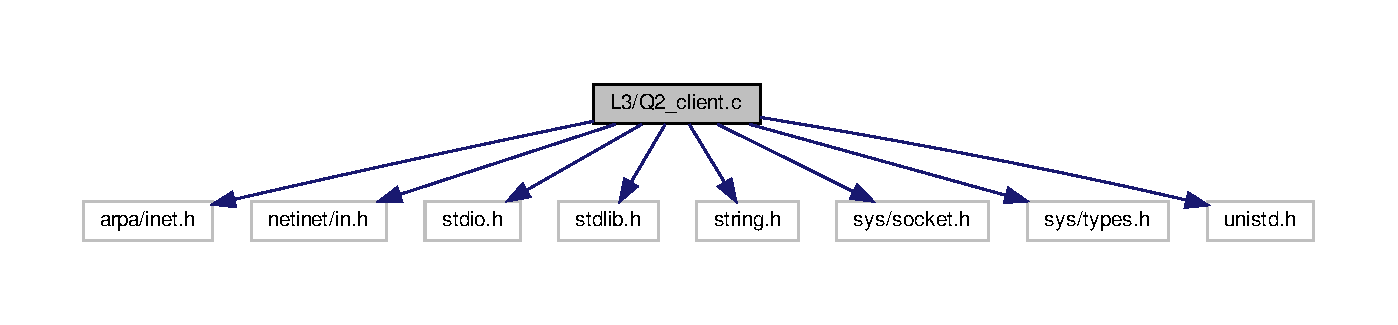
\includegraphics[width=350pt]{_q2__client_8c__incl}
\end{center}
\end{figure}
\subsection*{Macros}
\begin{DoxyCompactItemize}
\item 
\#define \hyperlink{_q2__client_8c_ac0a4ce3bd388c7823743b526e7cb77fb}{I\+P\+\_\+\+P\+R\+O\+T\+O\+C\+OL}~0
\item 
\#define \hyperlink{_q2__client_8c_ad8a262037cbfb38d1512f0073eeb7a66}{I\+P\+\_\+\+A\+D\+D\+R\+E\+SS}~\char`\"{}127.\+0.\+0.\+1\char`\"{}
\item 
\#define \hyperlink{_q2__client_8c_a47a4d3bbd05894abbce0ffd1d266aa88}{P\+O\+R\+T\+\_\+\+NO}~15050
\item 
\#define \hyperlink{_q2__client_8c_a30ba2113ad1b0f91029d017fc988d9af}{N\+E\+T\+\_\+\+B\+U\+F\+\_\+\+S\+I\+ZE}~32
\item 
\#define \hyperlink{_q2__client_8c_abace6f1e028b11cc237bd95c5dbe451a}{cipher\+Key}~\textquotesingle{}S\textquotesingle{}
\item 
\#define \hyperlink{_q2__client_8c_a6e618c0ec6ffc8ac4489d11c65a5a67c}{sendrecvflag}~0
\end{DoxyCompactItemize}
\subsection*{Functions}
\begin{DoxyCompactItemize}
\item 
void \hyperlink{_q2__client_8c_a37e9b2e0b0fcbe7d2d5bd9c9467c1fb8}{clear\+Buf} (char $\ast$b)
\item 
char \hyperlink{_q2__client_8c_a4fc6ad5854f646cf1e284f66e104219f}{Cipher} (char ch)
\item 
int \hyperlink{_q2__client_8c_a0d285ee71db2ee39e24c4a6e552991f3}{recv\+File} (char $\ast$buf, int s)
\item 
int \hyperlink{_q2__client_8c_ae66f6b31b5ad750f1fe042a706a4e3d4}{main} ()
\end{DoxyCompactItemize}


\subsection{Macro Definition Documentation}
\mbox{\Hypertarget{_q2__client_8c_abace6f1e028b11cc237bd95c5dbe451a}\label{_q2__client_8c_abace6f1e028b11cc237bd95c5dbe451a}} 
\index{Q2\+\_\+client.\+c@{Q2\+\_\+client.\+c}!cipher\+Key@{cipher\+Key}}
\index{cipher\+Key@{cipher\+Key}!Q2\+\_\+client.\+c@{Q2\+\_\+client.\+c}}
\subsubsection{\texorpdfstring{cipher\+Key}{cipherKey}}
{\footnotesize\ttfamily \#define cipher\+Key~\textquotesingle{}S\textquotesingle{}}



Definition at line 15 of file Q2\+\_\+client.\+c.

\mbox{\Hypertarget{_q2__client_8c_ad8a262037cbfb38d1512f0073eeb7a66}\label{_q2__client_8c_ad8a262037cbfb38d1512f0073eeb7a66}} 
\index{Q2\+\_\+client.\+c@{Q2\+\_\+client.\+c}!I\+P\+\_\+\+A\+D\+D\+R\+E\+SS@{I\+P\+\_\+\+A\+D\+D\+R\+E\+SS}}
\index{I\+P\+\_\+\+A\+D\+D\+R\+E\+SS@{I\+P\+\_\+\+A\+D\+D\+R\+E\+SS}!Q2\+\_\+client.\+c@{Q2\+\_\+client.\+c}}
\subsubsection{\texorpdfstring{I\+P\+\_\+\+A\+D\+D\+R\+E\+SS}{IP\_ADDRESS}}
{\footnotesize\ttfamily \#define I\+P\+\_\+\+A\+D\+D\+R\+E\+SS~\char`\"{}127.\+0.\+0.\+1\char`\"{}}



Definition at line 12 of file Q2\+\_\+client.\+c.

\mbox{\Hypertarget{_q2__client_8c_ac0a4ce3bd388c7823743b526e7cb77fb}\label{_q2__client_8c_ac0a4ce3bd388c7823743b526e7cb77fb}} 
\index{Q2\+\_\+client.\+c@{Q2\+\_\+client.\+c}!I\+P\+\_\+\+P\+R\+O\+T\+O\+C\+OL@{I\+P\+\_\+\+P\+R\+O\+T\+O\+C\+OL}}
\index{I\+P\+\_\+\+P\+R\+O\+T\+O\+C\+OL@{I\+P\+\_\+\+P\+R\+O\+T\+O\+C\+OL}!Q2\+\_\+client.\+c@{Q2\+\_\+client.\+c}}
\subsubsection{\texorpdfstring{I\+P\+\_\+\+P\+R\+O\+T\+O\+C\+OL}{IP\_PROTOCOL}}
{\footnotesize\ttfamily \#define I\+P\+\_\+\+P\+R\+O\+T\+O\+C\+OL~0}



Definition at line 11 of file Q2\+\_\+client.\+c.

\mbox{\Hypertarget{_q2__client_8c_a30ba2113ad1b0f91029d017fc988d9af}\label{_q2__client_8c_a30ba2113ad1b0f91029d017fc988d9af}} 
\index{Q2\+\_\+client.\+c@{Q2\+\_\+client.\+c}!N\+E\+T\+\_\+\+B\+U\+F\+\_\+\+S\+I\+ZE@{N\+E\+T\+\_\+\+B\+U\+F\+\_\+\+S\+I\+ZE}}
\index{N\+E\+T\+\_\+\+B\+U\+F\+\_\+\+S\+I\+ZE@{N\+E\+T\+\_\+\+B\+U\+F\+\_\+\+S\+I\+ZE}!Q2\+\_\+client.\+c@{Q2\+\_\+client.\+c}}
\subsubsection{\texorpdfstring{N\+E\+T\+\_\+\+B\+U\+F\+\_\+\+S\+I\+ZE}{NET\_BUF\_SIZE}}
{\footnotesize\ttfamily \#define N\+E\+T\+\_\+\+B\+U\+F\+\_\+\+S\+I\+ZE~32}



Definition at line 14 of file Q2\+\_\+client.\+c.

\mbox{\Hypertarget{_q2__client_8c_a47a4d3bbd05894abbce0ffd1d266aa88}\label{_q2__client_8c_a47a4d3bbd05894abbce0ffd1d266aa88}} 
\index{Q2\+\_\+client.\+c@{Q2\+\_\+client.\+c}!P\+O\+R\+T\+\_\+\+NO@{P\+O\+R\+T\+\_\+\+NO}}
\index{P\+O\+R\+T\+\_\+\+NO@{P\+O\+R\+T\+\_\+\+NO}!Q2\+\_\+client.\+c@{Q2\+\_\+client.\+c}}
\subsubsection{\texorpdfstring{P\+O\+R\+T\+\_\+\+NO}{PORT\_NO}}
{\footnotesize\ttfamily \#define P\+O\+R\+T\+\_\+\+NO~15050}



Definition at line 13 of file Q2\+\_\+client.\+c.

\mbox{\Hypertarget{_q2__client_8c_a6e618c0ec6ffc8ac4489d11c65a5a67c}\label{_q2__client_8c_a6e618c0ec6ffc8ac4489d11c65a5a67c}} 
\index{Q2\+\_\+client.\+c@{Q2\+\_\+client.\+c}!sendrecvflag@{sendrecvflag}}
\index{sendrecvflag@{sendrecvflag}!Q2\+\_\+client.\+c@{Q2\+\_\+client.\+c}}
\subsubsection{\texorpdfstring{sendrecvflag}{sendrecvflag}}
{\footnotesize\ttfamily \#define sendrecvflag~0}



Definition at line 16 of file Q2\+\_\+client.\+c.



\subsection{Function Documentation}
\mbox{\Hypertarget{_q2__client_8c_a4fc6ad5854f646cf1e284f66e104219f}\label{_q2__client_8c_a4fc6ad5854f646cf1e284f66e104219f}} 
\index{Q2\+\_\+client.\+c@{Q2\+\_\+client.\+c}!Cipher@{Cipher}}
\index{Cipher@{Cipher}!Q2\+\_\+client.\+c@{Q2\+\_\+client.\+c}}
\subsubsection{\texorpdfstring{Cipher()}{Cipher()}}
{\footnotesize\ttfamily char Cipher (\begin{DoxyParamCaption}\item[{char}]{ch }\end{DoxyParamCaption})}



Definition at line 27 of file Q2\+\_\+client.\+c.

\mbox{\Hypertarget{_q2__client_8c_a37e9b2e0b0fcbe7d2d5bd9c9467c1fb8}\label{_q2__client_8c_a37e9b2e0b0fcbe7d2d5bd9c9467c1fb8}} 
\index{Q2\+\_\+client.\+c@{Q2\+\_\+client.\+c}!clear\+Buf@{clear\+Buf}}
\index{clear\+Buf@{clear\+Buf}!Q2\+\_\+client.\+c@{Q2\+\_\+client.\+c}}
\subsubsection{\texorpdfstring{clear\+Buf()}{clearBuf()}}
{\footnotesize\ttfamily void clear\+Buf (\begin{DoxyParamCaption}\item[{char $\ast$}]{b }\end{DoxyParamCaption})}



Definition at line 19 of file Q2\+\_\+client.\+c.

\mbox{\Hypertarget{_q2__client_8c_ae66f6b31b5ad750f1fe042a706a4e3d4}\label{_q2__client_8c_ae66f6b31b5ad750f1fe042a706a4e3d4}} 
\index{Q2\+\_\+client.\+c@{Q2\+\_\+client.\+c}!main@{main}}
\index{main@{main}!Q2\+\_\+client.\+c@{Q2\+\_\+client.\+c}}
\subsubsection{\texorpdfstring{main()}{main()}}
{\footnotesize\ttfamily int main (\begin{DoxyParamCaption}{ }\end{DoxyParamCaption})}



Definition at line 49 of file Q2\+\_\+client.\+c.

\mbox{\Hypertarget{_q2__client_8c_a0d285ee71db2ee39e24c4a6e552991f3}\label{_q2__client_8c_a0d285ee71db2ee39e24c4a6e552991f3}} 
\index{Q2\+\_\+client.\+c@{Q2\+\_\+client.\+c}!recv\+File@{recv\+File}}
\index{recv\+File@{recv\+File}!Q2\+\_\+client.\+c@{Q2\+\_\+client.\+c}}
\subsubsection{\texorpdfstring{recv\+File()}{recvFile()}}
{\footnotesize\ttfamily int recv\+File (\begin{DoxyParamCaption}\item[{char $\ast$}]{buf,  }\item[{int}]{s }\end{DoxyParamCaption})}



Definition at line 33 of file Q2\+\_\+client.\+c.


\hypertarget{_q2__server_8c}{}\section{L3/\+Q2\+\_\+server.c File Reference}
\label{_q2__server_8c}\index{L3/\+Q2\+\_\+server.\+c@{L3/\+Q2\+\_\+server.\+c}}
{\ttfamily \#include $<$arpa/inet.\+h$>$}\newline
{\ttfamily \#include $<$netinet/in.\+h$>$}\newline
{\ttfamily \#include $<$stdio.\+h$>$}\newline
{\ttfamily \#include $<$stdlib.\+h$>$}\newline
{\ttfamily \#include $<$string.\+h$>$}\newline
{\ttfamily \#include $<$sys/socket.\+h$>$}\newline
{\ttfamily \#include $<$sys/types.\+h$>$}\newline
{\ttfamily \#include $<$unistd.\+h$>$}\newline
Include dependency graph for Q2\+\_\+server.\+c\+:
\nopagebreak
\begin{figure}[H]
\begin{center}
\leavevmode
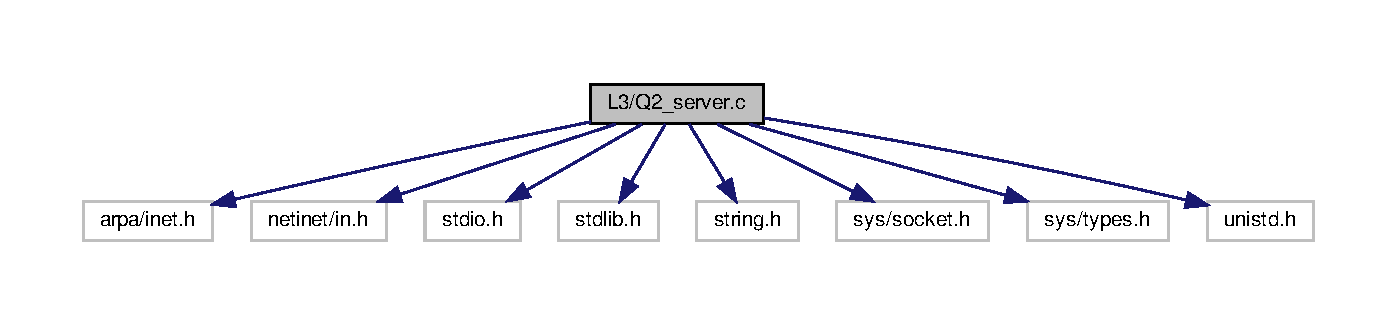
\includegraphics[width=350pt]{_q2__server_8c__incl}
\end{center}
\end{figure}
\subsection*{Macros}
\begin{DoxyCompactItemize}
\item 
\#define \hyperlink{_q2__server_8c_ac0a4ce3bd388c7823743b526e7cb77fb}{I\+P\+\_\+\+P\+R\+O\+T\+O\+C\+OL}~0
\item 
\#define \hyperlink{_q2__server_8c_a47a4d3bbd05894abbce0ffd1d266aa88}{P\+O\+R\+T\+\_\+\+NO}~15050
\item 
\#define \hyperlink{_q2__server_8c_a30ba2113ad1b0f91029d017fc988d9af}{N\+E\+T\+\_\+\+B\+U\+F\+\_\+\+S\+I\+ZE}~32
\item 
\#define \hyperlink{_q2__server_8c_abace6f1e028b11cc237bd95c5dbe451a}{cipher\+Key}~\textquotesingle{}S\textquotesingle{}
\item 
\#define \hyperlink{_q2__server_8c_a6e618c0ec6ffc8ac4489d11c65a5a67c}{sendrecvflag}~0
\item 
\#define \hyperlink{_q2__server_8c_a49e1fa6b4860231cbcb87bd74f65569f}{nofile}~\char`\"{}File Not Found!\char`\"{}
\end{DoxyCompactItemize}
\subsection*{Functions}
\begin{DoxyCompactItemize}
\item 
void \hyperlink{_q2__server_8c_a37e9b2e0b0fcbe7d2d5bd9c9467c1fb8}{clear\+Buf} (char $\ast$b)
\item 
char \hyperlink{_q2__server_8c_a4fc6ad5854f646cf1e284f66e104219f}{Cipher} (char ch)
\item 
int \hyperlink{_q2__server_8c_a19fc2d7afbfbca5d5b78534e8eeb6b29}{send\+File} (F\+I\+LE $\ast$fp, char $\ast$buf, int s)
\item 
int \hyperlink{_q2__server_8c_ae66f6b31b5ad750f1fe042a706a4e3d4}{main} ()
\end{DoxyCompactItemize}


\subsection{Macro Definition Documentation}
\mbox{\Hypertarget{_q2__server_8c_abace6f1e028b11cc237bd95c5dbe451a}\label{_q2__server_8c_abace6f1e028b11cc237bd95c5dbe451a}} 
\index{Q2\+\_\+server.\+c@{Q2\+\_\+server.\+c}!cipher\+Key@{cipher\+Key}}
\index{cipher\+Key@{cipher\+Key}!Q2\+\_\+server.\+c@{Q2\+\_\+server.\+c}}
\subsubsection{\texorpdfstring{cipher\+Key}{cipherKey}}
{\footnotesize\ttfamily \#define cipher\+Key~\textquotesingle{}S\textquotesingle{}}



Definition at line 23 of file Q2\+\_\+server.\+c.

\mbox{\Hypertarget{_q2__server_8c_ac0a4ce3bd388c7823743b526e7cb77fb}\label{_q2__server_8c_ac0a4ce3bd388c7823743b526e7cb77fb}} 
\index{Q2\+\_\+server.\+c@{Q2\+\_\+server.\+c}!I\+P\+\_\+\+P\+R\+O\+T\+O\+C\+OL@{I\+P\+\_\+\+P\+R\+O\+T\+O\+C\+OL}}
\index{I\+P\+\_\+\+P\+R\+O\+T\+O\+C\+OL@{I\+P\+\_\+\+P\+R\+O\+T\+O\+C\+OL}!Q2\+\_\+server.\+c@{Q2\+\_\+server.\+c}}
\subsubsection{\texorpdfstring{I\+P\+\_\+\+P\+R\+O\+T\+O\+C\+OL}{IP\_PROTOCOL}}
{\footnotesize\ttfamily \#define I\+P\+\_\+\+P\+R\+O\+T\+O\+C\+OL~0}



Definition at line 20 of file Q2\+\_\+server.\+c.

\mbox{\Hypertarget{_q2__server_8c_a30ba2113ad1b0f91029d017fc988d9af}\label{_q2__server_8c_a30ba2113ad1b0f91029d017fc988d9af}} 
\index{Q2\+\_\+server.\+c@{Q2\+\_\+server.\+c}!N\+E\+T\+\_\+\+B\+U\+F\+\_\+\+S\+I\+ZE@{N\+E\+T\+\_\+\+B\+U\+F\+\_\+\+S\+I\+ZE}}
\index{N\+E\+T\+\_\+\+B\+U\+F\+\_\+\+S\+I\+ZE@{N\+E\+T\+\_\+\+B\+U\+F\+\_\+\+S\+I\+ZE}!Q2\+\_\+server.\+c@{Q2\+\_\+server.\+c}}
\subsubsection{\texorpdfstring{N\+E\+T\+\_\+\+B\+U\+F\+\_\+\+S\+I\+ZE}{NET\_BUF\_SIZE}}
{\footnotesize\ttfamily \#define N\+E\+T\+\_\+\+B\+U\+F\+\_\+\+S\+I\+ZE~32}



Definition at line 22 of file Q2\+\_\+server.\+c.

\mbox{\Hypertarget{_q2__server_8c_a49e1fa6b4860231cbcb87bd74f65569f}\label{_q2__server_8c_a49e1fa6b4860231cbcb87bd74f65569f}} 
\index{Q2\+\_\+server.\+c@{Q2\+\_\+server.\+c}!nofile@{nofile}}
\index{nofile@{nofile}!Q2\+\_\+server.\+c@{Q2\+\_\+server.\+c}}
\subsubsection{\texorpdfstring{nofile}{nofile}}
{\footnotesize\ttfamily \#define nofile~\char`\"{}File Not Found!\char`\"{}}



Definition at line 25 of file Q2\+\_\+server.\+c.

\mbox{\Hypertarget{_q2__server_8c_a47a4d3bbd05894abbce0ffd1d266aa88}\label{_q2__server_8c_a47a4d3bbd05894abbce0ffd1d266aa88}} 
\index{Q2\+\_\+server.\+c@{Q2\+\_\+server.\+c}!P\+O\+R\+T\+\_\+\+NO@{P\+O\+R\+T\+\_\+\+NO}}
\index{P\+O\+R\+T\+\_\+\+NO@{P\+O\+R\+T\+\_\+\+NO}!Q2\+\_\+server.\+c@{Q2\+\_\+server.\+c}}
\subsubsection{\texorpdfstring{P\+O\+R\+T\+\_\+\+NO}{PORT\_NO}}
{\footnotesize\ttfamily \#define P\+O\+R\+T\+\_\+\+NO~15050}



Definition at line 21 of file Q2\+\_\+server.\+c.

\mbox{\Hypertarget{_q2__server_8c_a6e618c0ec6ffc8ac4489d11c65a5a67c}\label{_q2__server_8c_a6e618c0ec6ffc8ac4489d11c65a5a67c}} 
\index{Q2\+\_\+server.\+c@{Q2\+\_\+server.\+c}!sendrecvflag@{sendrecvflag}}
\index{sendrecvflag@{sendrecvflag}!Q2\+\_\+server.\+c@{Q2\+\_\+server.\+c}}
\subsubsection{\texorpdfstring{sendrecvflag}{sendrecvflag}}
{\footnotesize\ttfamily \#define sendrecvflag~0}



Definition at line 24 of file Q2\+\_\+server.\+c.



\subsection{Function Documentation}
\mbox{\Hypertarget{_q2__server_8c_a4fc6ad5854f646cf1e284f66e104219f}\label{_q2__server_8c_a4fc6ad5854f646cf1e284f66e104219f}} 
\index{Q2\+\_\+server.\+c@{Q2\+\_\+server.\+c}!Cipher@{Cipher}}
\index{Cipher@{Cipher}!Q2\+\_\+server.\+c@{Q2\+\_\+server.\+c}}
\subsubsection{\texorpdfstring{Cipher()}{Cipher()}}
{\footnotesize\ttfamily char Cipher (\begin{DoxyParamCaption}\item[{char}]{ch }\end{DoxyParamCaption})}

function to encrypt \begin{DoxyAuthor}{Author}
Aman Jaiswal 
\end{DoxyAuthor}

\begin{DoxyParams}{Parameters}
{\em character} & to encrypt \\
\hline
\end{DoxyParams}
\begin{DoxyDate}{Date}
22/08/2019 
\end{DoxyDate}


Definition at line 46 of file Q2\+\_\+server.\+c.

\mbox{\Hypertarget{_q2__server_8c_a37e9b2e0b0fcbe7d2d5bd9c9467c1fb8}\label{_q2__server_8c_a37e9b2e0b0fcbe7d2d5bd9c9467c1fb8}} 
\index{Q2\+\_\+server.\+c@{Q2\+\_\+server.\+c}!clear\+Buf@{clear\+Buf}}
\index{clear\+Buf@{clear\+Buf}!Q2\+\_\+server.\+c@{Q2\+\_\+server.\+c}}
\subsubsection{\texorpdfstring{clear\+Buf()}{clearBuf()}}
{\footnotesize\ttfamily void clear\+Buf (\begin{DoxyParamCaption}\item[{char $\ast$}]{b }\end{DoxyParamCaption})}

function to clear buffer \begin{DoxyAuthor}{Author}
Aman Jaiswal 
\end{DoxyAuthor}

\begin{DoxyParams}{Parameters}
{\em buffer} & b \\
\hline
\end{DoxyParams}
\begin{DoxyDate}{Date}
22/08/2019 
\end{DoxyDate}


Definition at line 33 of file Q2\+\_\+server.\+c.

\mbox{\Hypertarget{_q2__server_8c_ae66f6b31b5ad750f1fe042a706a4e3d4}\label{_q2__server_8c_ae66f6b31b5ad750f1fe042a706a4e3d4}} 
\index{Q2\+\_\+server.\+c@{Q2\+\_\+server.\+c}!main@{main}}
\index{main@{main}!Q2\+\_\+server.\+c@{Q2\+\_\+server.\+c}}
\subsubsection{\texorpdfstring{main()}{main()}}
{\footnotesize\ttfamily int main (\begin{DoxyParamCaption}{ }\end{DoxyParamCaption})}



Definition at line 81 of file Q2\+\_\+server.\+c.

\mbox{\Hypertarget{_q2__server_8c_a19fc2d7afbfbca5d5b78534e8eeb6b29}\label{_q2__server_8c_a19fc2d7afbfbca5d5b78534e8eeb6b29}} 
\index{Q2\+\_\+server.\+c@{Q2\+\_\+server.\+c}!send\+File@{send\+File}}
\index{send\+File@{send\+File}!Q2\+\_\+server.\+c@{Q2\+\_\+server.\+c}}
\subsubsection{\texorpdfstring{send\+File()}{sendFile()}}
{\footnotesize\ttfamily int send\+File (\begin{DoxyParamCaption}\item[{F\+I\+LE $\ast$}]{fp,  }\item[{char $\ast$}]{buf,  }\item[{int}]{s }\end{DoxyParamCaption})}

function sending file \begin{DoxyAuthor}{Author}
Aman Jaiswal 
\end{DoxyAuthor}

\begin{DoxyParams}{Parameters}
{\em buffer,fp} & file descriptor, \\
\hline
\end{DoxyParams}
\begin{DoxyDate}{Date}
22/08/2019 
\end{DoxyDate}


Definition at line 57 of file Q2\+\_\+server.\+c.


\hypertarget{ring_8tcl}{}\section{L3/ring.tcl File Reference}
\label{ring_8tcl}\index{L3/ring.\+tcl@{L3/ring.\+tcl}}
\subsection*{Functions}
\begin{DoxyCompactItemize}
\item 
\hyperlink{ring_8tcl_a30728837c246b65ef76298af0101d99c}{finish}
\end{DoxyCompactItemize}


\subsection{Function Documentation}
\mbox{\Hypertarget{ring_8tcl_a30728837c246b65ef76298af0101d99c}\label{ring_8tcl_a30728837c246b65ef76298af0101d99c}} 
\index{ring.\+tcl@{ring.\+tcl}!finish@{finish}}
\index{finish@{finish}!ring.\+tcl@{ring.\+tcl}}
\subsubsection{\texorpdfstring{finish()}{finish()}}
{\footnotesize\ttfamily finish}



Definition at line 11 of file ring.\+tcl.


\hypertarget{star_8tcl}{}\section{L3/star.tcl File Reference}
\label{star_8tcl}\index{L3/star.\+tcl@{L3/star.\+tcl}}
\subsection*{Functions}
\begin{DoxyCompactItemize}
\item 
\hyperlink{star_8tcl_a30728837c246b65ef76298af0101d99c}{finish}
\end{DoxyCompactItemize}


\subsection{Function Documentation}
\mbox{\Hypertarget{star_8tcl_a30728837c246b65ef76298af0101d99c}\label{star_8tcl_a30728837c246b65ef76298af0101d99c}} 
\index{star.\+tcl@{star.\+tcl}!finish@{finish}}
\index{finish@{finish}!star.\+tcl@{star.\+tcl}}
\subsubsection{\texorpdfstring{finish()}{finish()}}
{\footnotesize\ttfamily finish}



Definition at line 15 of file star.\+tcl.


%--- End generated contents ---

% Index
\backmatter
\newpage
\phantomsection
\clearemptydoublepage
\addcontentsline{toc}{chapter}{Index}
\printindex

\end{document}
